\chapter{Introducción}


\section{Contexto}


La industria del videojuego se ha consolidado durante las últimas décadas como uno de los sectores tecnológicos de mayor crecimiento a nivel mundial. En 2020, el mercado global de videojuegos generó ingresos estimados de 159.300 millones de dólares \cite{NEWZOO_GLOBAL_GAMES_MARKET_REPORT_2020_LIGHT}. Esta magnitud económica, unida a la constante evolución tecnológica del sector, convierte el desarrollo de videojuegos en un campo de estudio relevante para la ingeniería informática.

Desde la perspectiva de la ingeniería del software, el desarrollo de videojuegos plantea desafíos técnicos de considerable complejidad. Entre ellos destacan la arquitectura de sistemas en tiempo real, la implementación de algoritmos de inteligencia artificial, la generación procedural de contenido (creación automática de elementos del juego mediante algoritmos) y el diseño de interfaces interactivas. Este contexto convierte el desarrollo de un videojuego en un ámbito adecuado para la realización de un Trabajo de Fin de Grado (TFG) en Ingeniería Informática, al permitir la aplicación práctica e integrada de conocimientos adquiridos durante la formación académica en áreas como la programación orientada a objetos, las estructuras de datos, la arquitectura de software y la ingeniería del software.

Los videojuegos pertenecientes al subgénero \textit{roguelike} presentan una serie de características técnicas que los convierten en un objeto de estudio de especial interés desde el punto de vista de la ingeniería. Entre dichas características destacan la generación procedural de niveles, la ausencia de persistencia del progreso entre partidas -- lo que se conoce como \textit{permadeath} o muerte permanente --, la progresión limitada a cada ejecución del juego y una elevada rejugabilidad derivada de la variabilidad del contenido generado. Estas propiedades obligan a diseñar sistemas software capaces de producir escenarios jugables, coherentes y equilibrados de forma automática, sin intervención manual directa por parte de un diseñador de niveles.

En este contexto se plantea el siguiente problema técnico: cómo diseñar e implementar una arquitectura de software modular que permita la generación automática de niveles jugables, la gestión concurrente de múltiples subsistemas -- como la inteligencia artificial de los enemigos, el motor de físicas, la interfaz de usuario (UI) o el control de estados del juego -- y la parametrización del contenido de manera escalable y mantenible. Este problema resulta representativo de los retos que afronta la ingeniería del software aplicada al desarrollo de sistemas interactivos en tiempo real.

\section{Motivación y justificación}


La elección de un videojuego del subgénero \textit{roguelike} como objeto del presente Trabajo de Fin de Grado responde a una doble motivación: académica y técnica.

Desde el punto de vista académico, el desarrollo de un videojuego constituye un dominio de aplicación que permite integrar de forma práctica las competencias adquiridas a lo largo del Grado en Ingeniería Informática. En particular, el proyecto ofrece un marco adecuado para aplicar los contenidos estudiados en asignaturas clave de la titulación:

\begin{itemize}
\item \textbf{Ingeniería del Software (INSO).} Los patrones de diseño de software -- \textit{Singleton}, \textit{Observer}, \textit{Strategy} y \textit{Template Method} --, la captura de requisitos mediante historias de usuario, la arquitectura modular basada en la separación entre datos configurables y lógica de ejecución, y la gestión del ciclo de vida del software mediante una metodología iterativa e incremental constituyen contenidos propios de esta asignatura que se aplican de forma directa en el proyecto.
\item \textbf{Programación Orientada a Objetos.} La jerarquía de clases del sistema de enemigos (\texttt{Enemy} -> \texttt{SlimeGreen} / \texttt{SlimeRed} / \texttt{SlimeBlue}) y del sistema de armas (\texttt{Weapon} -> \texttt{MeleeWeapon} / \texttt{RangedWeapon}) aplica los principios de herencia, polimorfismo y encapsulamiento. El patrón \textit{Template Method}, que define comportamiento base en la clase padre y delega la especialización en las subclases, constituye un ejemplo representativo de la aplicación de estos conceptos.
\item \textbf{Algoritmia y Estructuras de Datos.} La generación procedural de salas, el algoritmo de expansión por \textit{clusters} (agrupaciones contiguas de tiles) para la distribución de tiles especiales, la generación ponderada de enemigos mediante presupuesto de coste y el control del flujo del juego mediante máquinas de estados constituyen problemas algorítmicos no triviales que permiten demostrar competencias en esta área.
\item \textbf{Diseño de Sistemas Interactivos.} La implementación de la interfaz de usuario -- sistema de corazones, menú de pausa, pantallas de fin de partida -- y la atención a la experiencia de juego mediante retroalimentación visual (parpadeo de invulnerabilidad, parpadeo rojo de muerte, efectos de impacto) se vinculan con los contenidos de diseño de interacción y usabilidad.
\end{itemize}

Esta vinculación con la Ingeniería del Software resulta especialmente significativa. El desarrollo de un videojuego \textit{roguelike} no se limita a la escritura de código: requiere definir una arquitectura de software modular, aplicar patrones de diseño reconocidos, gestionar la separación entre datos configurables y lógica de ejecución mediante mecanismos como los \textit{ScriptableObjects} (activos de datos serializables de Unity que permiten configurar parámetros desde el inspector del motor sin modificar el código fuente), y seguir una metodología de desarrollo que permita validar el producto de forma progresiva. Estos principios coinciden con los que articulan la disciplina de la Ingeniería del Software, lo que convierte el proyecto en un ejercicio representativo de las competencias que esta asignatura desarrolla.

Desde el punto de vista técnico, el subgénero \textit{roguelike} presenta una complejidad que lo convierte en un objeto de estudio adecuado para un Trabajo de Fin de Grado. La generación procedural de contenido obliga a diseñar algoritmos capaces de producir entornos jugables, coherentes y equilibrados sin intervención manual. La coordinación de múltiples subsistemas en tiempo real -- combate, inteligencia artificial, generación de niveles, interfaz de usuario -- exige una arquitectura con separación de responsabilidades y bajo acoplamiento entre componentes. Asimismo, la naturaleza iterativa del desarrollo de videojuegos, donde las mecánicas se ajustan mediante ciclos de prueba y refinamiento, se alinea con las metodologías de desarrollo incremental estudiadas durante la formación académica.

La relevancia cultural e industrial del subgénero refuerza la pertinencia de esta elección. Títulos como \textit{Hades} (Supergiant Games, 2020), \textit{Dead Cells} (Motion Twin, 2018), \textit{The Binding of Isaac} (Edmund McMillen, 2011) o \textit{Enter the Gungeon} (Dodge Roll, 2016) se han consolidado como referencias contemporáneas del subgénero. Por ejemplo, \textit{Hades} ha recibido reconocimiento en premios de la industria; en \textit{The Game Awards} 2020 obtuvo el galardón a Mejor Juego Independiente \cite{CNET_GAME_AWARDS_2020_WINNERS}. El análisis de estos sistemas permite abordar conceptos avanzados de ingeniería del software en un contexto práctico y representativo.

\section{Objetivos}


\subsection{Objetivo general}


El objetivo general del proyecto es diseñar, implementar y documentar un videojuego \textit{roguelike} funcional que permita evidenciar la aplicación de principios de ingeniería del software en el ámbito del desarrollo de videojuegos, con especial énfasis en la arquitectura modular y la generación procedural de contenido.

\subsection{Objetivos específicos}


De este objetivo general se derivan los siguientes objetivos específicos (OE):

\begin{enumerate}
\item \textbf{OE-1.} Diseñar e implementar una arquitectura modular basada en patrones de diseño (\textit{Singleton}, \textit{Observer}, \textit{Strategy}, \textit{Template Method}) que facilite la separación de responsabilidades entre subsistemas y promueva la mantenibilidad y extensibilidad del código.
\item \textbf{OE-2.} Desarrollar un algoritmo de generación procedural de salas que garantice la jugabilidad y la coherencia espacial del entorno, incluyendo la distribución de tiles especiales mediante clusters, la colocación de muros con colisionadores y el posicionamiento de escaleras de transición.
\item \textbf{OE-3.} Implementar tres comportamientos diferenciados de inteligencia artificial para los enemigos (persecución, ataque a distancia y aproximación por saltos) y un sistema de enemigos especiales con atributos escalados que actúen como jefes periódicos.
\item \textbf{OE-4.} Crear un sistema de armas con mecánicas de combate cuerpo a cuerpo y a distancia, incluyendo detección de colisiones, proyectiles físicos y un sistema de órbita del arma alrededor del jugador orientado hacia la posición del cursor.
\item \textbf{OE-5.} Implementar un sistema de tiles con efectos que modifiquen la jugabilidad, incluyendo su configuración mediante \textit{ScriptableObjects} y su distribución controlada en salas generadas proceduralmente.
\item \textbf{OE-6.} Implementar un sistema de persistencia de puntuaciones mediante \textit{PlayerPrefs} con visualización de un ranking en el menú principal, registrando estadísticas completas de cada partida.
\item \textbf{OE-7.} Documentar el proceso de desarrollo, las decisiones técnicas adoptadas y las limitaciones encontradas, exponiendo el trabajo realizado de forma rigurosa y reproducible.
\end{enumerate}

\section{Descripción del proyecto}


El videojuego desarrollado, denominado \textit{Ascension}, es un \textit{roguelike} bidimensional con vista cenital (\textit{top-down}, perspectiva en la que la cámara se sitúa sobre el escenario mirando hacia abajo), en el que el jugador avanza a través de una secuencia de salas generadas de forma procedural, enfrentándose a enemigos hasta alcanzar la condición de victoria establecida. Dicha condición consiste en la derrota de tres enemigos especiales con atributos incrementados -- denominados jefes -- que aparecen de forma periódica cada cinco salas completadas.

El sistema implementado incluye un flujo de juego completo que abarca las siguientes funcionalidades:

\begin{itemize}
\item \textbf{Menú principal} con acceso a la partida, tabla de puntuaciones y opción de salida.
\item \textbf{Selección de clase} entre tres personajes con estadísticas diferenciadas (vida máxima, velocidad de movimiento y arma inicial), lo que permite al jugador adaptar la experiencia a distintos estilos de juego.
\item \textbf{Gestión de estados globales} mediante un \textit{GameManager} (componente gestor central del juego) que coordina las transiciones entre menú, selección de clase, juego activo, pausa, victoria y derrota.
\item \textbf{Generación procedural de salas} mediante un \textit{RoomGenerator} que produce la estructura espacial de cada nivel basándose en \textit{tilemaps} con muros perimetrales, tiles de suelo con variantes visuales, tiles especiales con efectos (hielo, lodo, curación y potenciación de daño) y escaleras de transición entre salas.
\item \textbf{Sistema de combate} que contempla dos tipos de armas: cuerpo a cuerpo, cuyo ataque realiza un barrido angular con detección de colisión, y a distancia, que genera proyectiles físicos dirigidos hacia la posición del cursor. Ambos tipos de arma se configuran mediante \textit{ScriptableObjects} para su parametrización independiente del código.
\item \textbf{Inteligencia artificial de enemigos} con tres comportamientos diferenciados: persecución directa, ataque a distancia con mantenimiento de distancia óptima y aproximación por saltos (\textit{dash}, desplazamientos cortos y rápidos del enemigo hacia el jugador). Cada tipo de enemigo se configura mediante datos almacenados en \textit{ScriptableObjects}, lo que permite parametrizar atributos como velocidad, daño, vida y radio de detección.
\item \textbf{Sistema de gestión de enemigos} que utiliza un algoritmo de generación ponderada por coste, posicionamiento seguro respecto al jugador, limpieza automática de salas y control de interacción con las escaleras en función del estado del combate.
\item \textbf{Interfaz de usuario completa} con visualización dinámica de la salud del jugador mediante corazones, menú de pausa funcional y pantallas de victoria y derrota.
\item \textbf{Sistema de persistencia de puntuaciones} mediante \textit{PlayerPrefs} (almacenamiento local clave–valor proporcionado por Unity) y serialización JSON (\textit{JavaScript Object Notation}, conversión de estructuras de datos a texto estructurado), con un historial de hasta treinta partidas que registra puntuación, clase utilizada, salas completadas, enemigos eliminados, resultado y fecha.
\end{itemize}

El proyecto no incluye un sistema integral de audio ni un controlador genérico de objetos recolectables, al considerarse estos aspectos de menor prioridad para los objetivos académicos del trabajo. Asimismo, el sistema de jefes con fases múltiples y el sistema de generación de armas con rarezas constituyen funcionalidades preparadas a nivel de arquitectura para su extensión futura, pero no se encuentran completamente integradas en el flujo de juego durante la versión actual.

\section{Metodología}


\subsection{Tipo de investigación}


El trabajo se enmarca dentro de una investigación de tipo aplicado, centrada en el diseño e implementación de un producto software funcional. El objetivo principal es demostrar la aplicación práctica de conceptos propios de la ingeniería del software en el contexto del desarrollo de videojuegos, concretamente en la creación de un videojuego bidimensional del subgénero \textit{roguelike}.

\subsection{Metodología de desarrollo de software}


Se ha adoptado una metodología de desarrollo \textbf{iterativa e incremental}, basada en la implementación progresiva de funcionalidades completas y su validación iterativa. Esta decisión se justifica por dos razones fundamentales:

\begin{enumerate}
\item \textbf{Naturaleza exploratoria del proyecto.} El desarrollo de un videojuego requiere experimentar con mecánicas de juego, ajustar parámetros de balance y validar la jugabilidad de forma temprana. Una metodología secuencial (cascada) no permitiría esta flexibilidad.
\item \textbf{Necesidad de adaptación continua.} Durante el desarrollo se identificaron limitaciones técnicas y oportunidades de mejora que exigieron redefinir determinados aspectos del diseño. El enfoque iterativo permitió incorporar estos cambios sin comprometer la estabilidad del sistema.
\end{enumerate}

El proceso de trabajo se estructuró en \textbf{iteraciones de corta duración}, cada una de las cuales generó un incremento funcional del sistema. En cada iteración se llevaron a cabo las siguientes actividades:

\begin{enumerate}
\item \textbf{Diseño} de un subsistema concreto, definiendo su responsabilidad, sus interfaces y sus dependencias con otros módulos.
\item \textbf{Implementación} de la funcionalidad asociada, siguiendo los principios de separación de responsabilidades y bajo acoplamiento.
\item \textbf{Validación} mediante pruebas funcionales manuales en el editor de Unity, comprobando el funcionamiento del subsistema de forma aislada y su integración con los subsistemas existentes.
\item \textbf{Corrección} de errores detectados durante la validación.
\item \textbf{Ajuste del alcance} de iteraciones posteriores en función de los resultados obtenidos y de las prioridades identificadas.
\end{enumerate}

No se ha aplicado una metodología ágil formal como \textit{Scrum} o \textit{Kanban}, dado que el proyecto se ha desarrollado de manera individual. Sin embargo, el enfoque iterativo adoptado comparte principios fundamentales con las metodologías ágiles: entrega frecuente de incrementos funcionales, adaptación al cambio y validación iterativa del producto.

La elección del diseño iterativo se justifica por su adecuación al desarrollo de videojuegos, un ámbito en el que la experimentación, el ajuste de mecánicas y la validación temprana de funcionalidades son factores relevantes para favorecer la viabilidad del producto final y reducir el riesgo técnico. En la práctica, este enfoque permitió, por ejemplo, detectar la necesidad de implementar un sistema de gracia temporal (\textit{grace period}, un breve intervalo tras la aparición en el que el enemigo no puede dañar al jugador), evitando daño instantáneo antes de que el jugador pudiera reaccionar. Este tipo de ajustes, derivados de la validación funcional durante el desarrollo, habría sido difícil de anticipar en una fase de diseño inicial.

\subsection{Proceso de implementación y validación}


La implementación del sistema se llevó a cabo siguiendo un proceso de definición de subsistemas, codificación, pruebas funcionales y refinamiento. Cada componente del videojuego se desarrolló de forma modular e independiente y posteriormente se integró en el sistema global, comprobando su funcionamiento conjunto con los subsistemas ya existentes.

Las iteraciones de desarrollo se organizaron en torno a los siguientes subsistemas, implementados de forma secuencial con solapamientos parciales entre fases:

\begin{enumerate}
\item Gestión central del juego (\textit{GameManager}, máquina de estados, transiciones de escena).
\item Sistema de jugador (movimiento, esquiva, sistema de vida).
\item Generación procedural de salas (\textit{RoomGenerator}, \textit{tilemaps}, colisionadores).
\item Sistema de combate y armas (cuerpo a cuerpo, a distancia, proyectiles).
\item Inteligencia artificial de enemigos (tres comportamientos diferenciados).
\item Sistema de gestión de salas (flujo de progresión, enemigos especiales).
\item Sistema de tiles con efectos (hielo, lodo, curación, potenciación).
\item Interfaz de usuario (corazones, puntuación, menú de pausa, pantallas finales).
\item Sistema de persistencia (puntuaciones, historial de partidas).
\end{enumerate}

El proceso de validación se basó en pruebas funcionales manuales ejecutadas directamente en el editor de Unity. En cada iteración se comprobaron aspectos clave del sistema, entre los que se incluyen:

\begin{itemize}
\item La generación procedural de salas con muros de contención íntegros y área jugable accesible
\item El comportamiento de la inteligencia artificial de enemigos con distintos patrones de actuación
\item La aplicación correcta de efectos de tiles sobre el jugador y los enemigos
\item El flujo de avance entre salas y la aparición periódica de enemigos especiales
\item La activación de la condición de victoria tras la superación de los tres encuentros con jefes
\item La coherencia de la interfaz de usuario con el estado real del juego
\item La persistencia de puntuaciones entre sesiones de juego
\end{itemize}

No se realizó un proceso de pruebas de usuario con participantes externos. La validación durante el desarrollo se centró en comprobar la estabilidad funcional del sistema y detectar errores críticos durante las sesiones de juego realizadas.

\subsection{Ejemplos representativos de iteraciones y sus resultados}

Para ilustrar cómo la metodología iterativa e incremental influyó en las decisiones técnicas del proyecto, a continuación se describen tres situaciones concretas en las que la validación funcional de un incremento reveló problemas que motivaron cambios de diseño:

\begin{enumerate}
\item \textbf{Descubrimiento del sistema de gracia temporal.} Durante la iteración correspondiente al sistema de enemigos, las partidas de validación revelaron que los enemigos infligían daño al jugador en el mismo fotograma en que aparecían, antes de que el jugador pudiera reaccionar. Este problema no era visible en el diseño inicial -- que no contemplaba un retardo de activación -- pero resultaba evidente al jugar. Como resultado, se diseñó e implementó un sistema de periodos de gracia (\texttt{contactDamageGraceSeconds} y \texttt{aiGraceSeconds} de 0,75 segundos), que se integró en la clase base \texttt{Enemy} para que todos los tipos de enemigo lo heredasen automáticamente.
\item \textbf{Transición de generación de salas como escenas separadas a regeneración en la misma escena.} El diseño inicial contemplaba cargar una nueva escena de Unity para cada sala, lo que resultaba en tiempos de carga perceptibles (entre 0,5 y 1,5 segundos por transición, dependiendo de la complejidad de la escena) que rompían el ritmo de juego. La validación durante la iteración 3 evidenció este problema, y se rediseñó el sistema para regenerar el contenido del \textit{tilemap} dentro de la misma escena (\texttt{RegenerateFloorKeepWalls}), eliminando los tiempos de carga y manteniendo los colisionadores de muros intactos. Este cambio tuvo un impacto arquitectónico significativo: el \texttt{RoomFlowController} dejó de gestionar cargas de escena y pasó a coordinar directamente el \texttt{RoomGenerator} y el \texttt{EnemyManager} dentro de la escena activa.
\item \textbf{Limitador de velocidad de los enemigos.} Durante las pruebas del slime verde (francotirador), se detectó que en su estado de huida podía moverse más rápido que el jugador, lo que hacía imposible alcanzarlo. Este problema no se había previsto en el diseño porque la velocidad del enemigo y del jugador se configuraban de forma independiente en sus respectivos \textit{ScriptableObjects}. La solución fue implementar el método \texttt{CapToPlayerSpeed()}, que limita la velocidad efectiva de cualquier enemigo a un máximo igual a la velocidad actual del jugador, garantizando que la evasión nunca sea imposible.
\end{enumerate}

Estos tres casos ilustran el valor del enfoque iterativo: ninguno de los problemas habría sido detectado en una fase de diseño inicial, ya que solo se manifestaron durante la ejecución del juego con sistemas integrados.

\section{Planificación temporal}


\subsection{Estimación de la dedicación}


La dedicación total estimada del Trabajo de Fin de Grado asciende a 300 horas, distribuidas de forma desigual entre las distintas fases del proyecto según la naturaleza de las tareas.

\subsection{Fases del proyecto}


El proyecto se ha estructurado en las siguientes fases, con una estimación del esfuerzo dedicado a cada una:

\textbf{Fase 1. Investigación y definición de alcance (30 horas)}

Durante esta fase se realizó una exploración de posibles enfoques para el TFG, evaluando distintas ideas de proyecto y tecnologías. Se analizaron los requisitos generales del trabajo académico, se estudiaron las características del subgénero \textit{roguelike} y se llevó a cabo una primera toma de contacto con el motor Unity y el lenguaje C\#. Como resultado de esta fase se decidió orientar el TFG hacia el desarrollo de un videojuego del subgénero \textit{roguelike}, al considerarse un dominio adecuado para aplicar conocimientos de ingeniería del software. Se definieron los objetivos generales y específicos del proyecto.

\textbf{Fase 2. Diseño de arquitectura y prototipos iniciales (35 horas)}

En esta fase se diseñó la arquitectura inicial del sistema, definiendo los principales subsistemas del juego (gestión de estados, flujo de salas, generación procedural y combate) y estableciendo las bases del proyecto en Unity. Se tomaron decisiones técnicas clave relativas al uso de \textit{ScriptableObjects} para la parametrización de datos, la aplicación de patrones de diseño (\textit{Singleton}, \textit{Observer}) y la separación entre lógica de juego y datos configurables. Se implementaron prototipos funcionales del movimiento del jugador y de la generación básica de salas.

\textbf{Fase 3. Implementación del núcleo del juego (90 horas)}

Esta fase constituyó el núcleo del trabajo práctico. Se implementaron de forma incremental los sistemas fundamentales del videojuego:

\begin{itemize}
\item Sistema de generación procedural de salas con tiles, muros y colisionadores
\item Gestión del flujo de juego mediante \textit{RoomFlowController}
\item Sistema de combate con armas cuerpo a cuerpo y a distancia
\item Inteligencia artificial de los tres tipos de enemigos
\item Sistema de enemigos especiales con atributos escalados
\item Condición de victoria y derrota
\end{itemize}

La implementación se realizó de manera iterativa, validando la funcionalidad del juego en cada incremento y ajustando decisiones de diseño cuando fue necesario.

\textbf{Fase 4. Sistema de tiles, efectos e interfaz de usuario (40 horas)}

Se implementó el sistema de tiles especiales con efectos diferenciados (hielo, lodo, curación, potenciación de daño), incluyendo el algoritmo de distribución por clusters y la persistencia temporal de efectos. De forma paralela, se desarrolló la interfaz de usuario completa: sistema dinámico de corazones, indicador de puntuación, menú de pausa, pantallas de victoria y derrota, y tabla de puntuaciones con historial persistente.

\textbf{Fase 5. Ajuste de configuración y validación del contenido (30 horas)}

Se llevaron a cabo tareas de verificación y ajuste de configuraciones globales del proyecto (parámetros de importación de sprites, físicas, colisionadores y consistencia de activos), con el objetivo de reducir errores de configuración y facilitar la iteración sobre los contenidos del juego.

\textbf{Fase 6. Refinamiento, pruebas y depuración (20 horas)}

Se realizó un proceso de pruebas funcionales del sistema completo, comprobando la estabilidad del flujo de juego y corrigiendo errores detectados. Se llevaron a cabo ajustes de balance, mejoras en la interfaz de usuario y optimizaciones de rendimiento.

\textbf{Fase 7. Creación de assets gráficos (15 horas)}

Se diseñaron y crearon los sprites del juego, incluyendo los personajes jugables, los tres tipos de enemigos, las armas, los proyectiles, los tiles de suelo y muros, y los elementos de interfaz de usuario. Se utilizó la herramienta LibreSprite para la creación de \textit{pixel art} (técnica de creación de gráficos digitales en la que las imágenes se editan a nivel de píxel individual) a una resolución de 16 píxeles por unidad.

\textbf{Fase 8. Documentación y memoria (40 horas)}

Se redactó la memoria académica del Trabajo de Fin de Grado, documentando cada fase del proyecto, las decisiones técnicas adoptadas, la arquitectura del sistema, los módulos implementados, los patrones de diseño aplicados, los resultados obtenidos y las conclusiones alcanzadas. Se elaboraron los diagramas de clases, de secuencia y de Gantt incluidos en el documento.

\subsection{Representación gráfica de la planificación}


La Figura 1.1 muestra la planificación temporal del proyecto, con la distribución de las ocho fases, su dedicación en horas y la superposición parcial entre algunas de ellas.

\begin{figure}[H]
\begin{center}
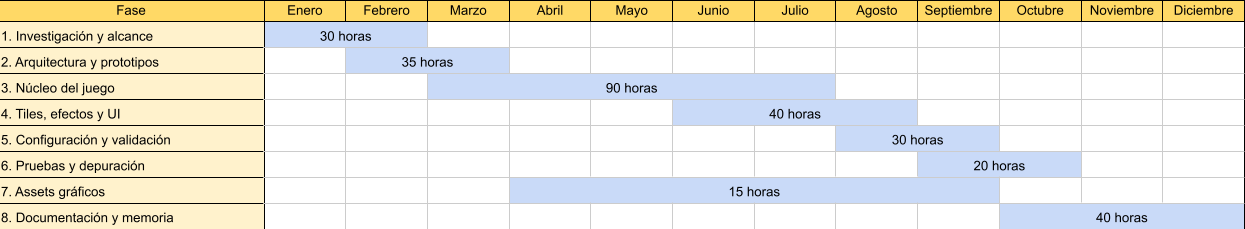
\includegraphics[width=0.95\textwidth]{Figuras/cronograma.png}
\caption{Diagrama de Gantt con la distribución temporal y la dedicación en horas de las ocho fases del proyecto (elaboración propia).}
\label{fig:gantt-planificacion}
\end{center}
\end{figure}


\section{Estructura de la memoria}


Esta memoria se organiza en seis capítulos. Tras la introducción, se analiza el estado del arte, referentes y tecnologías empleadas. Posteriormente, se detalla el diseño del sistema (requisitos y arquitectura) y su implementación técnica. Finalmente, se exponen las conclusiones y líneas de trabajo futuro.
